\documentclass[../../main.tex]{subfiles}
\begin{document}

{\bf [解]}

$t = e^x$ とおく．$x > 0$ から $t > 1$ である．
与えられた関数
\begin{align}
  f(x)=\dfrac{12(e^{3x}-3e^x)}{e^{2x}-1} = \dfrac{12(t^{3}-3t)}{t^{2}-1} \label{eq:1}
\end{align}
について考える．

\paragraph{(1)}

\cref{eq:1}の両辺を$x$で微分すると，合成微分から
\begin{align}
  f'(x)
  &= \dfrac{dt}{dx} \dfrac{df}{dt}
  = t \cdot \left\{ \dfrac{12(t^2 - 3t)}{(t^2 - 1)} \right\}' \\
  &= 12t \cdot \dfrac{t^4 + 3}{(t^2 - 1)^2} > 0 \quad (\because t > 1)
\end{align}
だから $f(x)$は単調増加である．
また，極限値は
\begin{align}
  \begin{cases}
    f(x) = 12 \dfrac{t - 3/t}{1 - 1/t^2} \xrightarrow{x \to \infty} \infty \quad (\because t \to \infty) \\
    f(x) = 12 \dfrac{t(t^2 - 3)}{(t+1)(t-1)} \xrightarrow{x \to +0} -\infty \quad (\because t \to 1+0)
  \end{cases}
\end{align}
だから，$f(x)$の増減表・グラフの概形は下のようになる．

% f(x)の増減表
\begin{table}[htb]
  \centering
  \caption{$f(x)$ の増減表 $(x > 0)$}
  \label{tab:fx_monotonicity}
  \renewcommand{\arraystretch}{1.5}
  \begin{tabular}{c|ccccc}
    \hline
    $x$      & $(0)$       & $\cdots$   & $\dfrac{1}{2}\log 3$ & $\cdots$   & $(\to\infty)$ \\ \hline
    $f'(x)$  & $(/)$       & $+$        & $+$                  & $+$        & $(/)$         \\ \hline
    $f(x)$   & $(-\infty)$ & $\nearrow$ & $0$                  & $\nearrow$ & $(\to\infty)$ \\ \hline
  \end{tabular}
\end{table}

% y=f(x)のグラフ
\begin{figure}[htb]
  \centering
  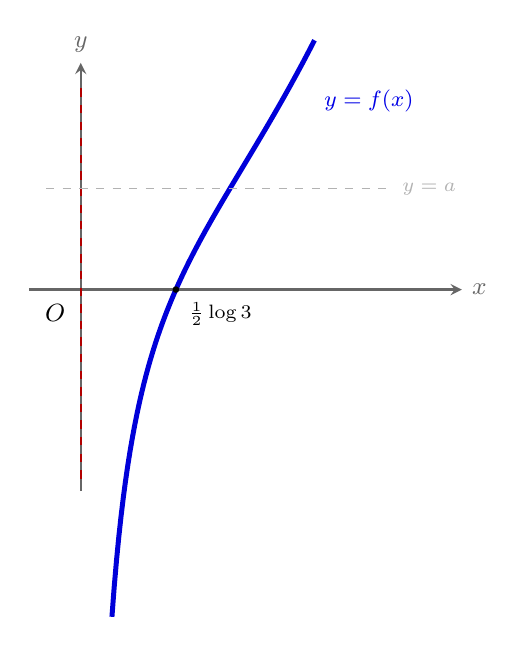
\begin{tikzpicture}[x=2.2cm, y=0.08cm, >=stealth, every node/.style={font=\small}]

    % --- 1. 定数・座標パラメータ ---
    % x_0 = 1/2 * log(3) ≈ 0.5493
    \pgfmathsetmacro{\xZero}{0.5 * ln(3)}

    % --- 2. 座標軸 ---
    \draw[->, thick, gray!80!black] (-0.3, 0) -- (2.2, 0) node[right] {$x$};
    \draw[->, thick, gray!80!black] (0, -32) -- (0, 36) node[above] {$y$};
    \node[below left=2pt] at (0, 0) {$O$};

    % --- 3. 漸近線 x = 0 (y 軸破線強調) ---
    \draw[dashed, red!70!black, thick] (0, -30) -- (0, 32);

    % --- 4. 曲線 y = f(x) のプロット ---
    % f(x) = 12*(exp(3x) - 3*exp(x))/(exp(2x) - 1)
    \draw[line width=1.8pt, blue!85!black, domain=0.18:1.35, samples=90]
    plot (\x, {12.0 * (exp(3.0*\x) - 3.0*exp(\x)) / (exp(2.0*\x) - 1.0)});
    \node[blue!90!black, font=\footnotesize\bfseries, right] at (1.35, 30) {$y = f(x)$};

    % --- 5. 特徴点・目盛り ---
    % x 軸との交点 (1/2 * log 3, 0)
    \fill[black] (\xZero, 0) circle (1.2pt);
    \node[below right=1pt, font=\scriptsize] at (\xZero, 0) {$\frac{1}{2}\log 3$};

    % 任意の定数 a の直線（解の唯一性の視覚化）
    \draw[dashed, gray!60] (-0.2, 16) -- (1.8, 16) node[right, font=\scriptsize] {$y = a$};

  \end{tikzpicture}
  \caption{$y = f(x)$ のグラフ}
  \label{fig:fx_monotonic_graph}
\end{figure}

従って任意の定数 $a$ に対し $f(x) = a$ なる $x > 0$ がただ1つある．

\paragraph{(2)}

% TODO: 面積Sの領域
\begin{figure}[htb]
  \centering
  \begin{tikzpicture}[x=3.8cm, y=0.15cm, >=stealth, every node/.style={font=\small}]

    % --- 1. 定数・厳密パラメータ ---
    % x_0 = 1/2 * log(3) ≈ 0.5493
    % x_1 = log(2)        ≈ 0.6931  (f(x_1) = 8)
    % x_2 = log(3)        ≈ 1.0986  (f(x_2) = 27)
    \pgfmathsetmacro{\xZero}{0.5 * ln(3)}
    \pgfmathsetmacro{\xOne}{ln(2)}
    \pgfmathsetmacro{\xTwo}{ln(3)}

    % 各頂点座標の定義
    \coordinate (O)     at (0, 0);
    \coordinate (D)     at (\xOne, 0);
    \coordinate (E)     at (\xOne, 8.0);
    \coordinate (F)     at (0, 8.0);
    \coordinate (A)     at (\xTwo, 0);
    \coordinate (B)     at (\xTwo, 27.0);
    \coordinate (C)     at (0, 27.0);

    % ============================================================
    % 2. 面積 S の斜線ハッチング (F -> E -> 曲線 -> B -> C -> F)
    % ============================================================
    \fill[pattern=north east lines, pattern color=blue!75, opacity=0.8]
    (F) -- (E)
    -- plot[domain=\xOne:\xTwo, samples=50]
    (\x, {12.0 * (exp(3.0*\x) - 3.0*exp(\x)) / (exp(2.0*\x) - 1.0)})
    -- (C) -- cycle;

    % ============================================================
    % 3. 座標軸
    % ============================================================
    \draw[->, thick, gray!80!black] (-0.15, 0) -- (1.45, 0) node[right] {$x$};
    \draw[->, thick, gray!80!black] (0, -4.0) -- (0, 33.0) node[above] {$y$};

    % ============================================================
    % 4. 曲線 y = f(x) のプロット
    % ============================================================
    \draw[line width=1.8pt, blue!85!black, domain=0.45:1.18, samples=70]
    plot (\x, {12.0 * (exp(3.0*\x) - 3.0*exp(\x)) / (exp(2.0*\x) - 1.0)});
    \node[blue!90!black, font=\footnotesize\bfseries, above right] at (1.1, 28) {$y = f(x)$};

    % ============================================================
    % 5. 投影破線 (長方形 OABC, ODEF の枠線)
    % ============================================================
    % y = 8, x = log 2
    \draw[dashed, gray!60, thick] (F) -- (E) -- (D);
    % y = 27, x = log 3
    \draw[dashed, gray!60, thick] (C) -- (B) -- (A);

    % ============================================================
    % 6. 各頂点のプロットとラベル (O, A, B, C, D, E, F)
    % ============================================================
    \fill[black] (O) circle (1.2pt) node[below left=2pt] {$O$};
    \fill[black] (A) circle (1.2pt) node[below=2pt] {$A(\log 3, 0)$};
    \fill[black] (B) circle (1.4pt) node[above right=1pt] {$B$};
    \fill[black] (C) circle (1.2pt) node[left=2pt] {$C(0, 27)$};
    \fill[black] (D) circle (1.2pt) node[below=2pt] {$D(\log 2, 0)$};
    \fill[black] (E) circle (1.4pt) node[below right=1pt] {$E$};
    \fill[black] (F) circle (1.2pt) node[left=2pt] {$F(0, 8)$};

    % x 軸との交点 (1/2 * log 3, 0)
    \fill[black] (\xZero, 0) circle (1.2pt);
    \node[below left=2pt, font=\scriptsize] at (\xZero, 0) {$\frac{1}{2}\log 3$};

    % 領域ラベル S
    \node[draw=blue!85!black, rounded corners=2pt, inner sep=3pt, font=\normalsize\bfseries, blue!90!black]
    at (0.35, 17.5) {$S$};

  \end{tikzpicture}
  \caption{$y = f(x)$ のグラフと $y = 8, 27$ で囲まれる面積 $S$（斜線部）}
  \label{fig:fx_area_S_rectangles}
\end{figure}

グラフの概形は上図で求める面積 $S$ は斜線部である．
各点を計算すると，
\begin{align}
  f(x) = 8
  &\iff 3t^3 - 2t^2 - 9t + 2 = 0 \\
  &\iff (t - 2)(3t^2 + 4t - 1) = 0 \\
  \therefore
  &t = 2 \quad (\because t > 1) \\
  %
  f(x) = 27
  &\iff 4t^3 - 9t^2 - 12t + 9 = 0 \\
  &\iff (t - 3)(4t^2 + 3t - 3) = 0 \\
  \therefore
  &t = 3 \quad (\because t > 1)
\end{align}
だから，$S$は
\begin{align}
  S
  &= \square OABC - \square ODEF - \text{図形}ABED \\
  &= 27 \log 3 - 8 \log 2 - \int_{\log 2}^{\log 3} f(x) dx \label{eq:2}
\end{align}
となる．第三項を計算すると
\begin{align}
  \int_{\log 2}^{\log 3} f(x) dx
  &= \int_2^3 \dfrac{12(t^3 - 3t)}{t^2 - 1} \dfrac{1}{t} dt \\
  &= 12 \int_2^3 \dfrac{t^2 - 3}{t^2 - 1} dt \\
  &= 12 \int_2^3 \left( 1 - \dfrac{1}{t - 1} + \dfrac{1}{t + 1} \right) dt \\
  &= 12 \Bigl[ t - \log(t-1) + \log(t+1) \Bigr]_2^3 \\
  &= 12(1 + \log 2 - \log 3)
\end{align}
だから，\cref{eq:2}に代入して求める面積は
\begin{align}
  S = 39 \log 3 - 20 \log 2 - 12
\end{align}
である．

{\bf [解2]}
\paragraph{(2)}

\cref{eq:2}は図形的な処理に頼らなくても置換積分で出てくる．
$S = \int_8^{27} g(x) dx$ とおく．$x = f(y)$ なる置換をして，
\begin{align}
  S
  &= \int_{\log 2}^{\log 3} y \cdot \dfrac{df(y)}{dy} dy \\
  &= \int_{\log 2}^{\log 3} y \cdot f'(y) dy \\
  &= \Bigl[ y f(y) \Bigr]_{\log 2}^{\log 3} - \int_{\log 2}^{\log 3} f(y) dy \\
  &= 27 \log 3 - 8 \log 2 - \int_{\log 2}^{\log 3} f(y) dy
\end{align}
であり，これは\cref{eq:2}と同じである．

\end{document}
